% preamble and style file for M&R lecture slides
\documentclass[11.5pt,sans,english]{beamer}

\usetheme{EastLansing}
\usecolortheme{lily}

\usepackage[most]{tcolorbox}

\usepackage{verbatim}
%\usepackage{ulem}
%\usepackage{fontawesome}
%\usepackage{tikz}
%\usepackage{pifont}
%\usepackage{tabularx}
\usepackage{array,booktabs,xcolor,colortbl,multirow,rotating,amssymb}
%\usepackage{amsmath}
% \usepackage{vwcol}
% \usepackage[T1]{fontenc}

  
\newcommand\vect[1]{\underline{\mathbf{#1}}}
\newcommand\unitvect[1]{\hat{\boldsymbol{#1}}}
%\newcommand\hatdot[1] { \hat{ \dot{ \boldsymbol{#1} } } }

\newtcbox
{\keyc}{on line,arc=2pt, colback=yellow!30!white, colframe=yellow!30!black, before upper={\rule[-3pt]{0pt}{10pt} },boxrule=1pt,boxsep=0pt,left=6pt,right=6pt,top=2pt,bottom=2pt,}

\newtcbox
{\keyb}{on line,arc=1pt, colback=blue!30!white, colframe=blue!30!black, before upper={\rule[-3pt]{0pt}{10pt} },boxrule=1pt,boxsep=0pt,left=6pt,right=6pt,top=2pt,bottom=2pt,}

\newtcbox
{\keyl}{on line,arc=1pt, colback=pink!30!white, colframe=blue!30!black, before upper={\rule[-3pt]{0pt}{10pt} },boxrule=1pt,boxsep=0pt,left=6pt,right=6pt,top=2pt,bottom=2pt,}

\newtcbox
{\keyw}{on line,arc=1pt, colback=red!30!white, colframe=blue!30!black, before upper={\rule[-3pt]{0pt}{10pt} },boxrule=1pt,boxsep=0pt,left=6pt,right=6pt,top=2pt,bottom=2pt,}

\newtcbox
{\keya}{on line,arc=1pt, colback=purple!30!white, colframe=blue!30!black, before upper={\rule[-3pt]{0pt}{10pt} },boxrule=1pt,boxsep=0pt,left=6pt,right=6pt,top=2pt,bottom=2pt,}

\newtcbox[auto counter,number within=section]
{keyf}
{
enhanced,
on line,
  boxsep=0pt,
  left=6pt,right=6pt,top=2pt,bottom=2pt,
  arc=5pt,
  boxrule=1pt,
  rightrule=38pt,
colback=green!10!white, 
colframe=green!50!black, 
title=\thetcbcounter,
detach title,
overlay unbroken and first ={
    \node[%rotate=90,
          %minimum width=1cm,
          anchor=south,
          font=\sffamily\bfseries\tiny,
          %yshift=-10pt,
          yshift=-5pt,
          xshift=-20pt,
          white]
    at (frame.east) {\thetcbcounter};
  }
}


\usepackage{xcolor}

%\usepackage{hyperref}
%\hypersetup{
%  pdfauthor={Lily Asquith},
%  urlcolor=blue,
%  colorlinks=true,
%  linkcolor=blue,
%  bookmarks=true
%}

%---------------------------------------------%
%              LILY'S COLOURS           %
%---------------------------------------------%
\definecolor{Wash}{RGB}{204,204,204}
%\definecolor{Pinky}{RGB}{254,200,254}%violet
\definecolor{Pinky}{RGB}{219,	240,	253}%violet
\definecolor{Bluey}{RGB}{0,190,255}%deep sky blue
\definecolor{DarkGrey}{RGB}{28,66,137}%dar grey
\definecolor{SussexWhite}{RGB}{253,255,254}%dar grey
\definecolor{LightGray}{RGB}{184,184,255}
\definecolor{YesGreen}{RGB}{0,128,0}
\definecolor{NoRed}{RGB}{250,0,0}



\definecolor{myred}{RGB}{255,153,153}
\definecolor{myorange}{RGB}{255,204,153}
\definecolor{myyellow}{RGB}{255,255,153}
\definecolor{mygreen}{RGB}{153,255,153}
\definecolor{mycyan}{RGB}{153,255,255}
\definecolor{myblue}{RGB}{153,204,255}
\definecolor{myviolet}{RGB}{153,153,255}
\definecolor{mypurple}{RGB}{204,153,255}
\definecolor{mypink}{RGB}{255,204,255}
\definecolor{mycoral}{RGB}{255,153,204}

%-----------------------------------------------------%
%              LILY'S COLUMN TYPES          %
%-----------------------------------------------------%
\newcolumntype{a}{>{\raggedright\arraybackslash}l}	
\newcolumntype{q}{>{\raggedright\arraybackslash}m{8cm}} 

%--------------------------------------------%
%              LILY'S SYMBOLS          %
%--------------------------------------------%
\newcommand{\dfinger}{\large{\textcolor{black}{\ding{43}}}\scriptsize}
\newcommand{\dstar}{\large{\textcolor{black}{\ding{76}}}\scriptsize}
\newcommand{\dwrite}{\large{\textcolor{black}{\ding{45}}}\scriptsize}
\newcommand{\ddiamond}{\small{\textcolor{DarkGrey}{\ding{117}}}\scriptsize}
\newcommand{\ddiamondwhite}{\small{\textcolor{SussexWhite}{\ding{117}}}\scriptsize}
\newcommand{\experiment}{\small{\textcolor{magenta}{\faCogs }}\scriptsize}
\newcommand{\watchit}{\textcolor{blue}{ \faYoutube}}


\makeatletter
\newcommand\notsotiny{\@setfontsize\notsotiny{6.5}{7.5}}
\makeatother


% 
\title[ Mechanics \& Relativity]{Mechanics \& Relativity}
%\subtitle{\textbf{Topic 1: Kinematics }}
\author[Dr Lily Asquith (Lily)]{ Dr Lily Asquith (Lily)}
\date[Week 6 content - delivered week 7]{Week 6 content - delivered week 7}
\logo{

\includegraphics[width=1.5cm]{../../utils/uslogo.jpg}
}


\begin{document}


\begin{frame}
\titlepage
\end{frame} 


\begin{frame}{Catch-up week}

\textit{Week 6 lectures were cancelled, so we are now doing the following}\\[1ex]

\textbf{Tuesday 9 Nov}: Energy \& Momentum lecture.\\[1ex]

\textbf{Weds 10 Nov}:  Rotation 1.\\[1ex]

\textbf{Thurs 11 Nov}:  Rotation 2.\\[1ex]

\textbf{Fri 12 Nov}:  \textcolor{red}{No submission required for Workshop 6 (Energy \& Momentum).}\\[1ex]

Please review the extra `mini-lectures' I am adding to canvas. Back to normal next week!\\[1ex]

\end{frame}

 \subsection{Potential Energy}


\begin{frame}{Forces Recap}

\small

The Gravitational force (near Earth's surface)\\[2ex]
The Spring force (for springs obeying Hooke's law)\\[2ex]
Applied forces\\[2ex]
The normal force\\[2ex]
The centripetal force\\[2ex]
Frictional forces\\[2ex]
The drag force\\[2ex]

%The first two on this list are special: they are conservative.\\
%A conservative force does not create sound, heat.\\

\vspace{10cm}
\end{frame}




\begin{frame}{Work Recap}

\small
Work done by:\\[2ex]
Gravitational force (on/near Earth's surface)\\[2ex]
Spring force \\[2ex]
Applied forces\\[2ex]
The normal force\\[2ex]
The centripetal force\\[2ex]
Frictional forces\\[2ex]
The drag force\\[2ex]



\vspace{10cm}
\end{frame}


\begin{frame}{The truth about gravity}
\small
%$\vect{F}_g = - mg \unitvect{j}$ is an approximation. \\[2ex]
%$\vect{F}_G=\frac{mMG}{\vect{r}^2}$ is the full formula.\\[2ex]
%Because we live on Earth's surface, our distance from its centre is essentially constant.\\[2ex]
%G and M are constant.\\[2ex]
%So we use `little g': $g = \frac{MG}{r^2}$\\[2ex]

\vspace{10cm}
The gravitational force is variable with distance, just like the spring force.\\


\end{frame}


\begin{frame}{Conservative Forces}
\small
Integrate to get the work done by the force in moving a particle from the initial to final position:\\[1ex]
Spring force: \\[8ex]
Gravitational force: \\[8ex]


This work is a form of energy that cannot be lost to heat or sound. It is conserved.\\
The path of the object is irrelevant if the only force(s) conservative.\\


\end{frame}

\begin{frame}{Potential Energy}
\small
The potential energy of a system is increased if work is done in the opposite direction to that of the force.\\[2ex]

In the case of gravity, we set our zero point to be at Earth's surface:\\[15ex]


In the case of springs, we set our zero point to be at equilibrium:\\[15ex]


\end{frame}



 \subsection{Energy Conservation}

\begin{frame}{Mechanical Energy Conservation}
\small

A child of mass m is released from rest at the top of a water slide, at height $h~=~8.5$ m above the bottom of the slide. Assuming that the slide is frictionless because of the water on it, find the child's speed at the bottom of the slide.\\[2ex]




%Total Energy:\\[8ex]


\vspace{10cm}
\end{frame}

\begin{frame}{Another example}
\small
A small block of mass m = 0.032 kg can slide along a frictionless loop-the-loop, with loop radius R = 12 cm. The block is released from rest at point P, at height h = 5.0R above the bottom of the loop. How much work does the gravitational force do on the block as the block travels from point P to (a) point Q and (b) the top of the loop? \\
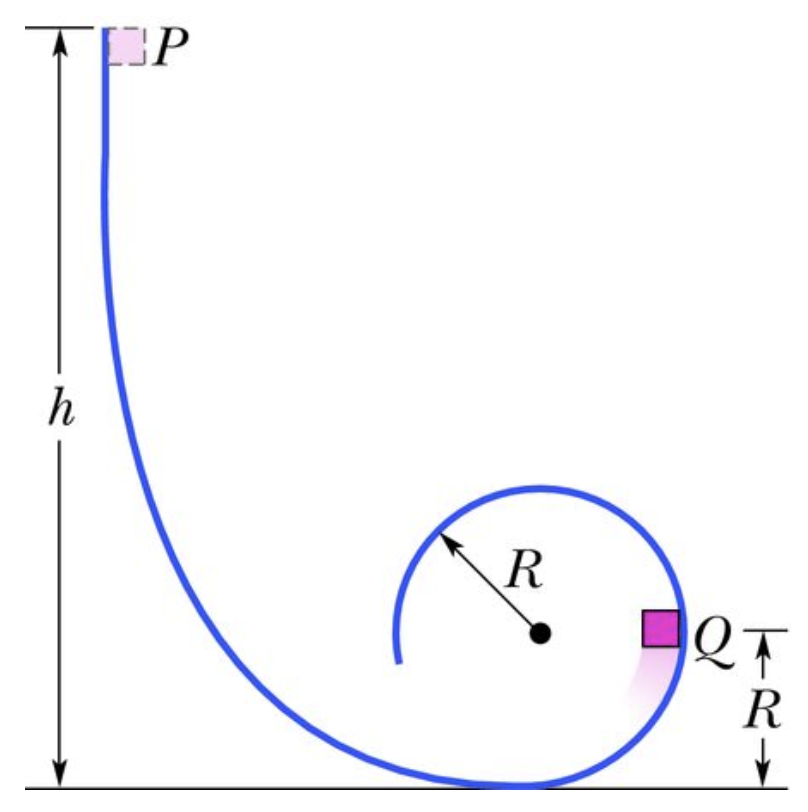
\includegraphics[scale=0.3]{loop}
%If the gravitational potential energy of the block?Earth system is taken to be zero at the bottom of the loop, what is that potential energy when the block is (c) at point P, (d) at point Q, and (e) at the top of the loop? (f) If, instead of merely being released, the block is given some initial speed downward along the track, do the answers to (a) through (e) increase, decrease, or remain the same?
\vspace{5cm}
\end{frame}






 \subsection{Linear Momentum \& Collisions}

\begin{frame}{Linear Momentum }
\small
Momentum $ \vect{p} = m \vect{v} $\\[1ex]
$ \vect{F} = m \vect{a} = m\frac{d\vect{v} }{dt} = \frac{d\vect{p} }{dt}$ \\[2ex]

For a closed, isolated system, $\vect{p}$ is always conserved.\\[1ex]

Total linear Momentum (a vector) is conserved, even when mechanical energy (a scalar) is not...\\
  
\vspace{10cm}
\end{frame}



\begin{frame}{Using conservation of $\vect{p}$ }
\small
A space hauler and cargo module, of total mass M, traveling along an x axis in deep space. They have an initial velocity of magnitude 2100 km/h relative to the Sun. With a small explosion, the hauler ejects the cargo module, of mass 0.20M. The hauler then travels 500 km/h faster than the module along the x axis; that is, the relative speed between the hauler and the module is 500 km/h. What then is the velocity of the hauler relative to the Sun?
\vspace{8cm}

\end{frame}

\begin{frame}{Types of Collisions}
\small
A totally elastic collision is one in which the KE is conserved  (as well as the linear momentum):\\[4ex]

An  inelastic collision is one in which the KE is not conserved  (but linear momentum is):\\[4ex]

A totally inelastic collision is a special case where two bodies become one:\\[4ex]

\end{frame}



\begin{frame}{Linear Momentum \& Collisions}
\small
A 0.165 kg cue ball as it bounces from a rail of a pool table. The ball's initial speed is 2.00 ms$^{-1}$, and the angle $\theta_1 = 30.0^{\circ}$. The bounce reverses the y component of the ball?s velocity but does not alter the x component. What are (a) angle $\theta_2$ and (b) the change in the ball's linear momentum in unit-vector notation? 
\vspace{10cm}
%What kind of collision is this?\\

\end{frame}



\begin{frame}{Linear Momentum \& Collisions}
\small
Suppose a gangster sprays Superman's chest with 3g bullets at the rate of 100 bullets/min, and the speed of each bullet is 500 m/s. Suppose too that the bullets rebound straight back with no change in speed. What is the magnitude of the average force on Superman's chest?
\vspace{10cm}
\end{frame}





\end{document}